\section{External interface requirements}
\label{sec:external_interface_requirements}%

\subsection{User interfaces}
\label{subsec:User_interfaces}%
The S\&C system will be a web app accessible by different devices and form factors, with a responsive UI. The UI will be different based on the type of user, reflecting the different functionalities they need. Every user will need to insert their credentials to have access to the platform and there will be a mechanism to recover them in case of a loss. The UI will comply with accessibility standards to ensure usability for all users, including those with disabilities.

\subsection{Hardware interfaces}
\label{subsec:hardware_interfaces}%
Our platform is a web app, as a consequence, it does not require any specific hardware
interface. Users only need a device with a browser to access the website and an internet connection. Latest versions of browsers are suggested to ensure compatibility and optimal performance. The user is free to choose his device but accessing the web app from a desktop form factor is strongly recommended for the best user experience.


\subsection{Software interfaces}
\label{subsec:software_interfaces}%
No specific software interfaces are needed. However, a mailing system to send confirmation emails will be used to the users during the registration process. In the future, integrations with university and company tools will be possible to enhance interoperability.

\subsection{Communication interfaces}
\label{subsec:communication_interfaces}%
The communication interfaces needed by the system include the HTTPS protocol for secure data transfer between the client and server. SSL/TLS certificates will ensure encrypted communication to protect user credentials and sensitive information.

\section{Functional requirements}
\label{sec:functional_requirements}%

\subsection{Requirements}
\label{subsec:requirements3}%
\newcounter{req}
\setcounter{req}{1}
\newcommand{\creq}{\thereq\stepcounter{req}}
\begin{center}
    \begin{longtable}{|l|p{0.9\linewidth}|}
        \hline
        \textbf{ID} & \textbf{Description}\\
        \hline
        R\creq & {The system allows STs to register by providing personal information, email, and a password.}\\
        \hline
        R\creq & {The system shall allow Users to log in using their credentials.}\\
        \hline
        R\creq & {The system shall allow STs to edit their profiles, including personal details and contact information.}\\
        \hline
        R\creq & {The system shall enforce role-based access control to restrict access to specific functionalities based on the user type (ST, CP, UV).}\\
        \hline
        R\creq & {The system shall allow CPs to post new internship opportunities, including position details, required skills, duration, and compensation.}\\
        \hline
        R\creq & {The system shall allow STs to apply for internships by submitting a CV and optional cover letter.}\\
        \hline
        R\creq & {The system shall notify CPs when STs apply to an internship.}\\
        \hline
        R\creq & {The system shall allow CPs to review applications and schedule interviews with STs.}\\
        \hline
        R\creq & {The system shall allow CPs to submit questionnaires to STs.}\\
        \hline
        R\creq & {The system shall allow CPs to accept or reject applications and notify STs of the decision.}\\
        \hline
        R\creq & {The system shall allow UVs to manage their students and monitor their activity.}\\
        \hline
        R\creq & {The system shall send notifications to users for events such as application submissions, approvals, or rejections.}\\
        \hline
        R\creq & {The system shall allow CPs to track the progress of STs during the internship and provide regular feedback.}\\
        \hline
        R\creq & {The system shall allow CPs to evaluate the performance of STs at the end of the internship.}\\
        \hline
        R\creq & {The system shall allow UVs to review the feedback and evaluation provided by both CPs and STs.}\\
        \hline
        R\creq & {The system shall allow STs to search for internships using keywords, filters, or location.}\\
        \hline
        R\creq & {The system shall recommend internships to STs based on their skills, preferences, and past applications.}\\
        \hline
        R\creq & {The system shall recommend STs to CPs for specific internships based on their skills, preferences, and past applications.}\\
        \hline
        R\creq & {The system shall allow CPs to search for suitable STs based on their skills, academic background, and CVs.}\\
        \hline
        R\creq & {The system shall maintain a database of all internships, applications, and evaluations.}\\
        \hline
        \caption{Requirements.}
        \label{tab: requirements}%
    \end{longtable}
\end{center}

\subsection{Use case diagrams}
\label{subsec:use_case_diagrams}%

\begin{figure}[H]
    \begin{center}
        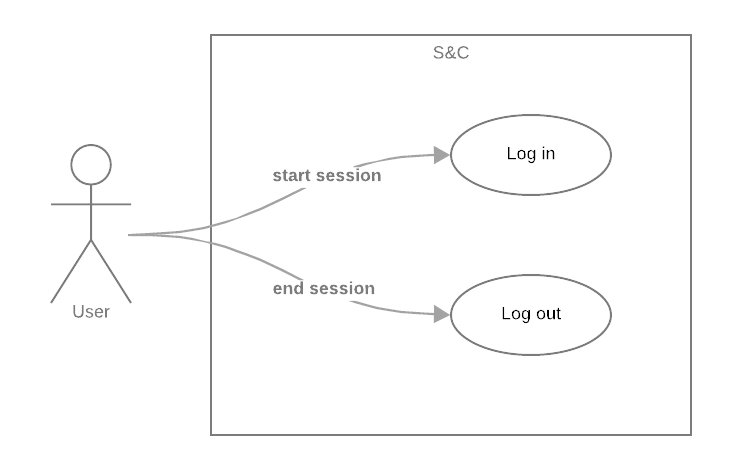
\includegraphics[width=0.8\linewidth]{UseCaseDiagrams/User.png}
        \caption{Use Cases Diagram for all users.} 
        \label{fig:UserUC}%
    \end{center}
\end{figure}

\begin{figure}[H]
    \begin{center}
        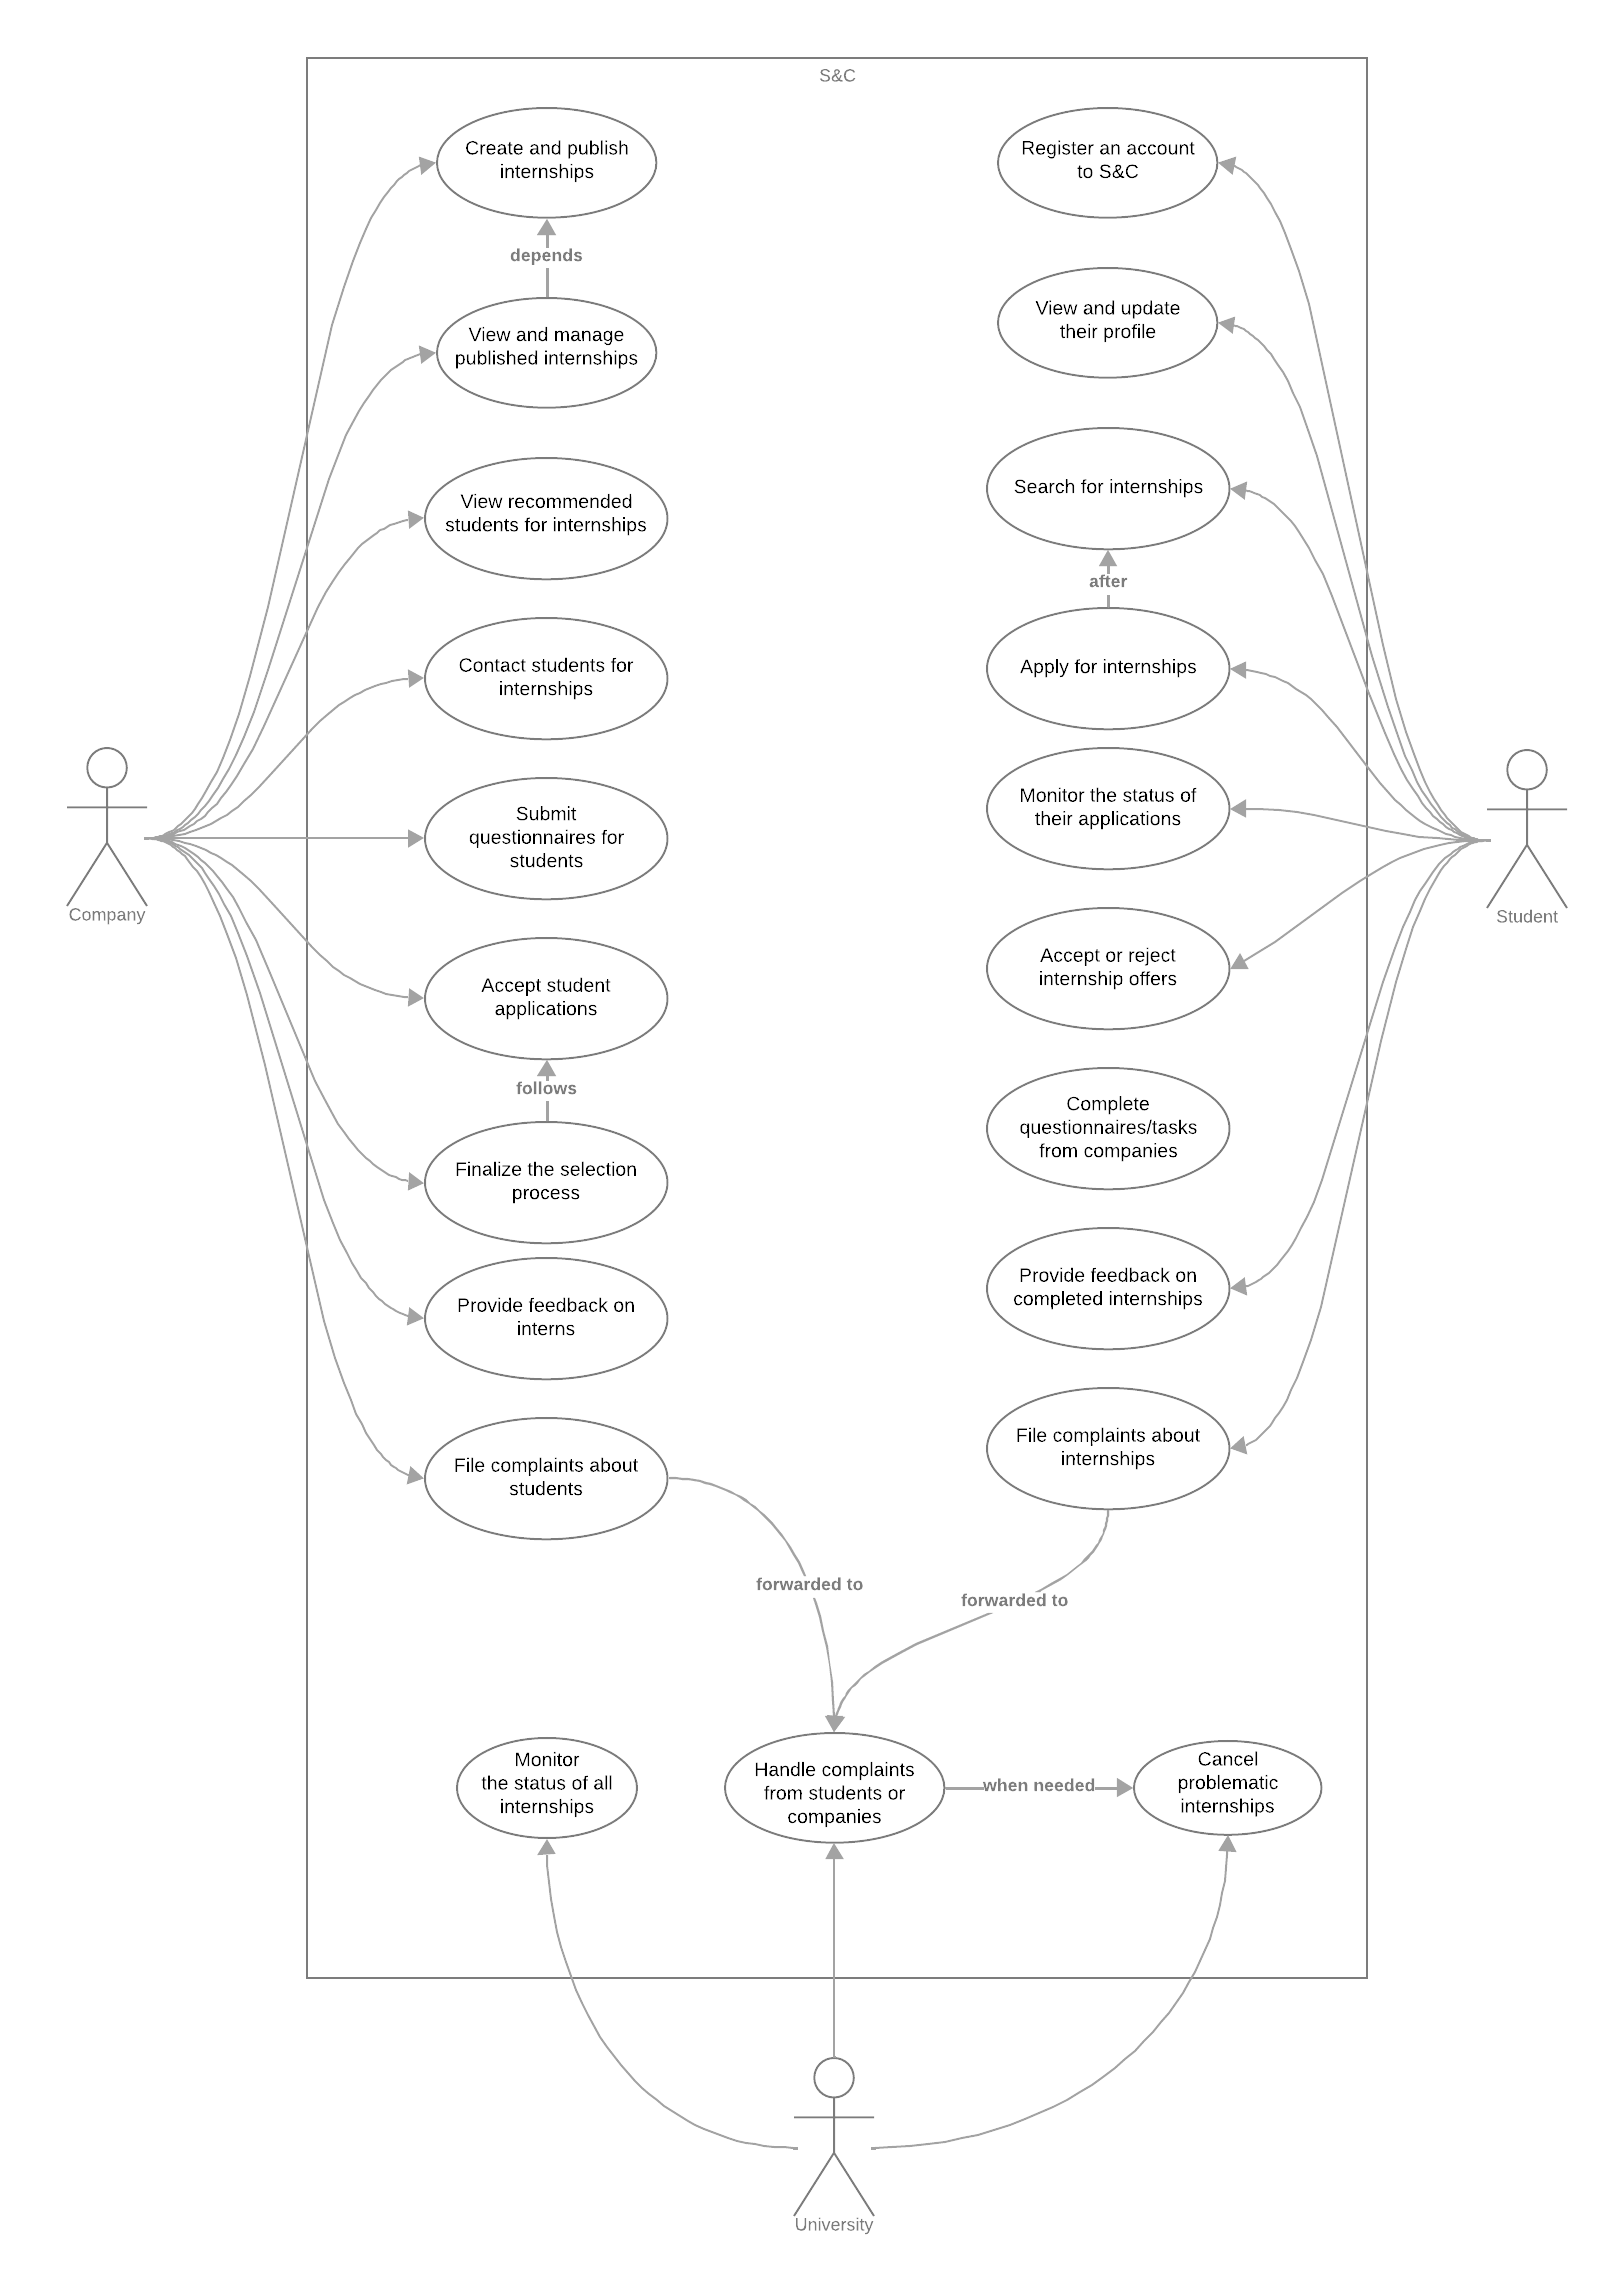
\includegraphics[width=\linewidth]{UseCaseDiagrams/Company_Student_University.png}
        \caption{Use Cases Diagram for company, student and university.} 
        \label{fig:Company_Student_UniversityUC}%
    \end{center}
\end{figure}

\begin{figure}[H]
    \begin{center}
        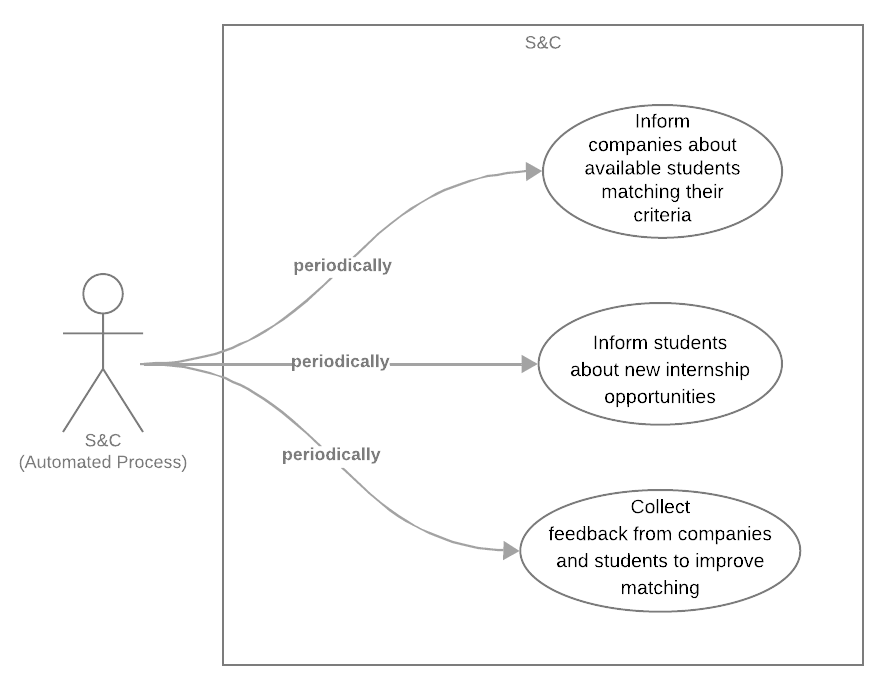
\includegraphics[width=0.8\linewidth]{UseCaseDiagrams/SeC.png}
        \caption{Use Cases Diagram for S\&C.} 
        \label{fig:SeCUC}%
    \end{center}
\end{figure}

\newpage
\subsection{Use cases}
\label{subsec: use_cases}%
\newcounter{uc}
\setcounter{uc}{1}
\newcommand{\cuc}{\theuc\stepcounter{uc}}
This section explains the main use cases and how they work. It includes a table for each use case that shows the starting conditions, steps involved, ending conditions, and any exceptions. There's also a sequence diagram that illustrates the messages exchanged between different entities and the functions that are called. \\

\subsubsection*{UC\cuc . Log in to the system}
\begin{center}
    \begin{longtable}{|l|p{0.75\linewidth}|}
        \hline
        \textbf{Actor}            & Student (ST), Company (CP), University (UV) \\
        \hline
        \textbf{Entry conditions} & The user has valid credentials (email and password) and access to S\&C's login page. \\
        \hline
        \textbf{Event Flow}       & 1 - The user navigates to the login page. \\
                                  & 2 - The user inputs their email and password. \\
                                  & 3 - S\&C validates the credentials. \\
                                  & 4 - The user is redirected to their respective dashboard. \\
        \hline
        \textbf{Exit condition}   & The user is logged into S\&C and has access to their dashboard. \\       
        \hline
        \textbf{Exceptions}       & - Incorrect email or password: The system displays an error message. \\
                                  & - System unavailable: S\&C informs the user and retries later. \\
        \hline
        \caption{Log in to the system}
        \label{tab:login_usecase}
    \end{longtable}
\end{center}

\begin{figure}[H]
    \begin{center}
        \includesvg[width=\textwidth]{SequenceDiagrams/Login.svg}
        \caption{Log in to the system sequence diagram.}
        \label{fig:login_seqd}%
    \end{center}
\end{figure}

\subsubsection*{UC\cuc . Log out from the system}
\begin{center}
    \begin{longtable}{|l|p{0.75\linewidth}|}
        \hline
        \textbf{Actor}            & Student (ST), Company (CP), University (UV) \\
        \hline
        \textbf{Entry conditions} & The user is logged into S\&C and has access to their dashboard. \\
        \hline
        \textbf{Event Flow}       & 1 - The user clicks the "Log Out" button. \\
                                  & 2 - S\&C invalidates the user's session. \\
                                  & 3 - S\&C redirects the user to the login page. \\
        \hline
        \textbf{Exit condition}   & The user is logged out of S\&C and redirected to the login page. \\       
        \hline
        \textbf{Exceptions}       & - System unavailable: S\&C informs the user and retries later. \\
        \hline
        \caption{Log out from the system}
        \label{tab:logout_usecase}
    \end{longtable}
\end{center}

\begin{figure}[H]
    \begin{center}
        \includesvg[width=0.8\textwidth]{SequenceDiagrams/Logout.svg}
        \caption{Log out from the system sequence diagram.}
        \label{fig:logout_seqd}%
    \end{center}
\end{figure}

\subsubsection*{UC\cuc . Register an account to S\&C}
FATTO DA MIRKO SU DRRIVE

\subsubsection*{UC\cuc . View and update their profile}
\begin{center}
    \begin{longtable}{|l|p{0.75\linewidth}|}
        \hline
        \textbf{Actor}            & Student (ST) \\
        \hline
        \textbf{Entry conditions} & The student is logged into S\&C. \\
        \hline
        \textbf{Event Flow}       & 1 - The user navigates to the profile section. \\
        & 2 - The user views their profile details. \\
        & 3 - The user updates specific fields (e.g., contact info, skills, CV). \\
        & 4 - S\&C validates the changes. \\
        & 5 - S\&C saves the updated profile. \\
        \hline
        \textbf{Exit condition}   & The user's profile is updated and saved successfully. \\       
        \hline
        \textbf{Exceptions}       & - Invalid data: S\&C prompts the user to correct the information. \\
                                  & - System unavailable: S\&C informs the user and retries later. \\
        \hline
        \caption{View and update their profile}
        \label{tab:view_update_profile_usecase}
    \end{longtable}
\end{center}

\begin{figure}[H]
    \begin{center}
        \includesvg[width=0.9\textwidth]{SequenceDiagrams/View_And_Update.svg}
        \caption{View and update profile sequence diagram.}
        \label{fig:view_update_profile_seqd}%
    \end{center}
\end{figure}

\subsubsection*{UC\cuc . Search for internships}
\begin{center}
    \begin{longtable}{|l|p{0.75\linewidth}|}
        \hline
        \textbf{Actor}            & Student (ST) \\
        \hline
        \textbf{Entry conditions} & The user is logged into S\&C. \\
        \hline
        \textbf{Event Flow}       & 1 - The user navigates to the internships section. \\
        & 2 - The user searches (e.g. by keywords, location, filters). \\
        & 3 - S\&C processes the search and retrieves results. \\
        & 4 - The user views the list of available internships. \\
        \hline
        \textbf{Exit condition}   & The user views relevant internship opportunities. \\       
        \hline
        \textbf{Exceptions}       & - No results: S\&C informs the user that no internships match the criteria. \\
                                  & - System unavailable: S\&C informs the user and retries later. \\
        \hline
        \caption{Search for internships}
        \label{tab:search_internships_usecase}
    \end{longtable}
\end{center}

\begin{figure}[H]
    \begin{center}
        \includesvg[width=\textwidth]{SequenceDiagrams/Search_Internships.svg}
        \caption{Search for internships sequence diagram.}
        \label{fig:search_internships_seqd}%
    \end{center}
\end{figure}

\subsubsection*{UC\cuc . Apply for an internship}
\begin{center}
    \begin{longtable}{|l|p{0.75\linewidth}|}
        \hline
        \textbf{Actor}            & Student (ST) \\
        \hline
        \textbf{Entry conditions} & The user is logged into S\&C and has selected an internship. \\
        \hline
        \textbf{Event Flow}       & 1 - The user navigates to the internship details page. \\
        & 2 - The user clicks the "Apply" button. \\
        & 3 - S\&C validates the user's eligibility. \\
        & 4 - S\&C submits the application. \\
        & 5 - S\&C confirms the application to the user. \\
        \hline
        \textbf{Exit condition}   & The user's application is successfully submitted. \\       
        \hline
        \textbf{Exceptions}       & - Not eligible: S\&C notifies the user with the reason for ineligibility (e.g. does not have the necessary skills). \\
                                  & - System unavailable: S\&C informs the user and retries later. \\
        \hline
        \caption{Apply for an internship}
        \label{tab:apply_internship_usecase}
    \end{longtable}
\end{center}

\begin{figure}[H]
    \begin{center}
        \includesvg[width=0.9\textwidth]{SequenceDiagrams/Apply_Internship.svg}
        \caption{Apply for an internship sequence diagram.}
        \label{fig:apply_internship_seqd}%
    \end{center}
\end{figure}

\subsubsection*{UC\cuc . Monitor the status of their applications}
\begin{center}
    \begin{longtable}{|l|p{0.75\linewidth}|}
        \hline
        \textbf{Actor}            & Student (ST) \\
        \hline
        \textbf{Entry conditions} & The user is logged into S\&C and has submitted at least one application. \\
        \hline
        \textbf{Event Flow}       & 1 - The user navigates to the "My Applications" section. \\
        & 2 - S\&C retrieves the status of all submitted applications. \\
        & 3 - The user views the list of applications and their statuses. \\
        \hline
        \textbf{Exit condition}   & The user views the status of their applications. \\       
        \hline
        \textbf{Exceptions}       & - No applications: S\&C informs the user that no applications have been submitted. \\
                                  & - System unavailable: S\&C informs the user and retries later. \\
        \hline
        \caption{Monitor the status of their applications}
        \label{tab:monitor_status_applications_usecase}
    \end{longtable}
\end{center}

\begin{figure}[H]
    \begin{center}
        \includesvg[width=0.9\textwidth]{SequenceDiagrams/Monitor_Status.svg}
        \caption{Monitor the status of their applications sequence diagram.}
        \label{fig:monitor_status_seqd}%
    \end{center}
\end{figure}

\subsubsection*{UC\cuc . Accept or reject internship offers}
\begin{center}
    \begin{longtable}{|l|p{0.75\linewidth}|}
        \hline
        \textbf{Actor}            & Student (ST) \\
        \hline
        \textbf{Entry conditions} & The user is logged into S\&C. \\
        \hline
        \textbf{Event Flow}       & 1 - The user navigates to the "Offers" section. \\
        & 2 - S\&C retrieves the list of received offers. \\
        & 3 - The user selects an offer to review. \\
        & 4 - The user chooses to accept or reject the offer. \\
        & 5 - S\&C updates the offer status. \\
        \hline
        \textbf{Exit condition}   & The offer status is updated as accepted or rejected. \\       
        \hline
        \textbf{Exceptions}       & - No offers available: S\&C notifies the user. \\
                                  & - Offer expired: S\&C notifies the user. \\
                                  & - System unavailable: S\&C informs the user and retries later. \\
        \hline
        \caption{Accept or reject internship offers}
        \label{tab:accept_reject_offers_usecase}
    \end{longtable}
\end{center}

\begin{figure}[H]
    \begin{center}
        \includesvg[width=0.9\textwidth]{SequenceDiagrams/Accept_Reject_Offers.svg}
        \caption{Accept or reject internship offers sequence diagram.}
        \label{fig:accept_reject_offers_seqd}%
    \end{center}
\end{figure}

\subsubsection*{UC\cuc . Complete questionnaires from companies}
FATTO DA MIRKO SU DRIVE

\subsubsection*{UC\cuc . Provide feedback on completed internships}
\begin{center}
    \begin{longtable}{|l|p{0.75\linewidth}|}
        \hline
        \textbf{Actor}            & Student (ST) \\
        \hline
        \textbf{Entry conditions} & The user is logged into S\&C and has completed at least one internship. \\
        \hline
        \textbf{Event Flow}       & 1 - The user navigates to the "Completed Internships" section. \\
        & 2 - S\&C retrieves the list of completed internships. \\
        & 3 - The user selects an internship to provide feedback on. \\
        & 4 - The user fills out the feedback form. \\
        & 5 - S\&C saves the user's feedback. \\
        \hline
        \textbf{Exit condition}   & Feedback for the internship is successfully submitted. \\       
        \hline
        \textbf{Exceptions}       & - System unavailable: S\&C informs the user and retries later. \\
        \hline
        \caption{Provide feedback on completed internships}
        \label{tab:provide_feedback_usecase}
    \end{longtable}
\end{center}

\begin{figure}[H]
    \begin{center}
        \includesvg[width=1\textwidth]{SequenceDiagrams/Provide_Feedback.svg}
        \caption{Provide feedback on completed internships sequence diagram.}
        \label{fig:provide_feedback_seqd}%
    \end{center}
\end{figure}

\subsubsection*{UC\cuc . File complaints about internships}
\begin{center}
    \begin{longtable}{|l|p{0.75\linewidth}|}
        \hline
        \textbf{Actor}            & Student (ST) \\
        \hline
        \textbf{Entry conditions} & The user is logged into S\&C and has encountered an issue with an internship. \\
        \hline
        \textbf{Event Flow}       & 1 - The user navigates to the "Complaints" section. \\
        & 2 - S\&C provides the complaint form. \\
        & 3 - The user fills out the complaint form, describing the issue. \\
        & 4 - The user submits the complaint. \\
        & 5 - S\&C saves and forwards the complaint to the relevant parties. \\
        \hline
        \textbf{Exit condition}   & The complaint is successfully filed and acknowledged by S\&C. \\       
        \hline
        \textbf{Exceptions}       & - System unavailable: S\&C informs the user and retries later. \\
        \hline
        \caption{File complaints about internships}
        \label{tab:file_complaints_usecase}
    \end{longtable}
\end{center}

\begin{figure}[H]
    \begin{center}
        \includesvg[width=1\textwidth]{SequenceDiagrams/File_Complaints.svg}
        \caption{File complaints about internships sequence diagram.}
        \label{fig:file_complaints_seqd}%
    \end{center}
\end{figure}

\subsubsection*{UC\cuc . Create and publish internships}
\begin{center}
    \begin{longtable}{|l|p{0.75\linewidth}|}
        \hline
        \textbf{Actor}            & Company (CP)\\
        \hline
        \textbf{Entry conditions} & The CP is correctly logged in. The CP has decided to create a internship. The CP is on his profile page. \\
        \hline
        \textbf{Event Flow}     & 1 - The CP clicks on "Publish a Internship"                                button.\\
                                & 2 - S\&C returns the publish internship form.\\
                                & 3 - The CP writes the internship name, specify the application domain, tasks to be performed, relevant adopted technologies ad terms offered\\
                                & 4 - S\&C stores the data of the internship and add it to the CP's internship list\\
                                & 5 - S\&C sends a notication to the STs that might be interested.\\
        \hline
        \textbf{Exit condition}   & The internship is correctly created and a confirmation message is shown to the CP. \\       
        \hline
        \textbf{Exceptions}       & - The internship's information are not                                  correct (internship's name null or already                                exist, some parameter inserted with not correct                           format). An error message is shown and the CP                             is redirected back to the publish internship                              form.\\
        \hline
        \caption{Create and publish internships}
        \label{tab: create_and_publish_internships_usecase}
    \end{longtable}
\end{center}

\begin{figure}[H]
    \begin{center}
        \includesvg[width=\textwidth]{SequenceDiagrams/Create_Internship.svg}
        \caption{Create and publish internships sequence diagram.}
        \label{fig:create_internship_seqd}%
    \end{center}
\end{figure}

\subsubsection*{UC\cuc . View and manage published internships}
FATTO DA MIRKO SU DRIVE

\subsubsection*{UC\cuc . View recommended students for internships}
\begin{center}
    \begin{longtable}{|l|p{0.75\linewidth}|}
        \hline
        \textbf{Actor}            & Company (CP)\\
        \hline
        \textbf{Entry conditions} & The company is logged into S\&C and has at least one published internship.\\
        \hline
        \textbf{Event Flow}     & 1 - The company navigates to the "Published                              Internships" section. \\
                                & 2 - S\&C retrieves the list of internships published by the company. \\
                                & 3 - The company selects an internship to view its details. \\
                                & 4 - S\&C retrieves internship's details and the list of suggested students.\\
        \hline
        \textbf{Exit condition}     & The company successfully views the list of                                suggested students.\\       
        \hline
        \textbf{Exceptions}     & - No recommended students: S\&C informs the company that there aren't recommended students. \\
                                & - System unavailable: S\&C logs the issue and retries later. \\
        \hline
        \caption{View recommended students for internships}
        \label{tab: view_recommended_students_for_internships_usecase}
    \end{longtable}
\end{center}

\begin{figure}[H]
    \begin{center}
        \includesvg[width=\textwidth]{SequenceDiagrams/View_Recommended_Students.svg}
        \caption{View recommended students for internships sequence diagram.}
        \label{fig:view_recommended_students_seqd}%
    \end{center}
\end{figure}

\subsubsection*{UC\cuc . Contact students for internships}
\begin{center}
    \begin{longtable}{|l|p{0.75\linewidth}|}
        \hline
        \textbf{Actor}            & Company (CP)\\
        \hline
        \textbf{Entry conditions} & The company is logged into S\&C. The company should be on a specific internship page to select a student’s name from the recommended students list.\\
        \hline
        \textbf{Event Flow}     & 1 - The company click on a student's name. \\
                                & 2 - S\&C returns the profile page of the selected student. \\
                                & 3 - The company click on the "invite" button. \\
                                & 4 - S\&C sends to the student a request of application.\\
                                & 5 - S\&C redirect the company to the "Progress Page" of the application.\\
        \hline
        \textbf{Exit condition}     & The company successfully views profile of                                the student and sends correctly the notification.\\       
        \hline
        \textbf{Exceptions}     & - Student profile not existing: S\&C informs company that the profile of the selected student is no longer available. \\
                                & - System unavailable: S\&C logs the issue and retries later. \\
        \hline
        \caption{Contact students for internships}
        \label{tab: contact_students_for_internships_usecase}
    \end{longtable}
\end{center}

\begin{figure}[H]
    \begin{center}
        \includesvg[width=\textwidth]{SequenceDiagrams/Contact_Students.svg}
        \caption{Contact students for internships sequence diagram.}
        \label{fig:contact_students_for_internships_seqd}%
    \end{center}
\end{figure}

\subsubsection*{UC\cuc . Accept student applications}
\begin{center}
    \begin{longtable}{|l|p{0.75\linewidth}|}
        \hline
        \textbf{Actor}            & Company (CP)\\
        \hline
        \textbf{Entry conditions} & The company is logged into S\&C. The company wants to review apply requests.\\
        \hline
        \textbf{Event Flow}     & 1 - The company navigates to the "Published                                                        Internships" section. \\
                                & 2 - S\&C retrieves the list of internships published by the company. \\
                                & 3 - The company selects an internship to view its details. \\
                                & 4 - S\&C retrieves internship's details and the list of apply requests.\\
                                & 5 - Company click on the students name.\\
                                & 6 - S\&C returns the profile page of the selected student.\\
                                & 7 - Company check the profile of the student and his CV.\\
                                & 8 - Company decide to accept or reject the apply request.\\
                                & 9 - S\&C send a notification to the student with the company’s decision.\\
                                & 10 - If the company has accepted, S\&C authorizes the assignment of tasks by the company.\\
        \hline
        \textbf{Exit condition}     & The company successfully accept the request and the student receive the notification.\\       
        \hline
        \textbf{Exceptions}     & - Student profile not existing: S\&C informs company that the profile of the selected student is no longer available. \\
                                & - System unavailable: S\&C logs the issue and retries later. \\
        \hline
        \caption{Accept student applications}
        \label{tab: accept_student_applications_usecase}
    \end{longtable}
\end{center}

\begin{figure}[H]
    \begin{center}
        \includesvg[width=\textwidth]{SequenceDiagrams/Accept_Student_Applications.svg}
        \caption{Accept student applications sequence diagram.}
        \label{fig:accept_student_applications_seqd}%
    \end{center}
\end{figure}

\subsubsection*{UC\cuc . Submit questionnaires for students}
\begin{center}
    \begin{longtable}{|l|p{0.75\linewidth}|}
        \hline
        \textbf{Actor}            & Company (CP)\\
        \hline
        \textbf{Entry conditions} & The company is logged into S\&C. The company wants to send questionnaires to students.\\
        \hline
        \textbf{Event Flow}     & 1 - The company goes to a student’s application "Progress Page". \\
                                & 2 - The company click the "create task" button. \\
                                & 3 - S\&C returns the task form.\\
                                & 4 - Company fill the form with task’s requirements, delivery instruction and deadline.\\
                                & 5 -  S\&C adds task to the Progress Page of the application and notify the ST about new assignments.\\
        \hline
        \textbf{Exit condition}     & The company successfully add the task and the student receive the notification.\\       
        \hline
        \textbf{Exceptions}     & - Data inserted by the company incomplete: an error message is shown and the CP is redirected back to the task form. \\
                                & - System unavailable: S\&C logs the issue and retries later. \\
        \hline
        \caption{Submit questionnaires for students}
        \label{tab: submit_questionnaires_for_students_usecase}
    \end{longtable}
\end{center}

\begin{figure}[H]
    \begin{center}
        \includesvg[width=\textwidth]{SequenceDiagrams/Submit_Questionnaires_Students.svg}
        \caption{Submit questionnaires for students sequence diagram.}
        \label{fig:submit_questionnaires_for_students_seqd}%
    \end{center}
\end{figure}

\subsubsection*{UC\cuc . Finalize the selection process}
\begin{center}
    \begin{longtable}{|l|p{0.75\linewidth}|}
        \hline
        \textbf{Actor}            & Company (CP)\\
        \hline
        \textbf{Entry conditions} & The company is logged into S\&C. The company wants to finalize the selection process.\\
        \hline
        \textbf{Event Flow}    & 1 - The company navigates to the "Published                                                        Internships" section. \\
                                & 2 - S\&C retrieves the list of internships published by the company. \\
                                & 3 - The company selects an internship to view its details. \\
                                & 4 - S\&C retrieves internship's details and the list of applicant students.\\
                                & 5 - The company selects students.\\
                                & 6 - S\&C add selected student to the internship’s list and notifies both selected and rejected students.\\
        \hline
        \textbf{Exit condition}     & The company successfully select the students and all the students receive the notification.\\       
        \hline
        \textbf{Exceptions}     & - One student profile not existing: S\&C informs company that the profile of the selected student is no longer available.\\
                                & - System unavailable: S\&C logs the issue and retries later. \\
        \hline
        \caption{Finalize the selection process}
        \label{tab: finalize_the_selection_process_usecase}
    \end{longtable}
\end{center}

\begin{figure}[H]
    \begin{center}
        \includesvg[width=\textwidth]{SequenceDiagrams/Finalize_Selection_Process.svg}
        \caption{Finalize the selection process sequence diagram.}
        \label{fig:finalize_the_selection_process_seqd}%
    \end{center}
\end{figure}

\subsubsection*{UC\cuc . Provide feedback on interns}
FATTO DA MIRKO SU DRIVE

\subsubsection*{UC\cuc . File complaints about students}
FATTO DA MIRKO SU DIVE

\subsubsection*{UC\cuc . Monitor the status of all internships}
TODO

\subsubsection*{UC\cuc . Handle complaints from students or companies}
TODO

\subsubsection*{UC\cuc . Cancel problematic internships}
TODO

\subsubsection*{UC\cuc . Collect feedback from companies and students to improve matching}
TODO

\subsubsection*{UC\cuc . Inform companies about available students matching their criteria}
FATTO DA MIRKO SU DRIVE

\subsubsection*{UC\cuc . Inform students about new internship opportunities}
FATTO DA MIRKO SU DRIVE

\newpage

\subsection{Requirement mapping}
\label{subsec:requirement_mapping}%
\textbf{G1 - Allow companies to post their internship opportunities.}
\begin{itemize}
    \item R2: The system shall allow Users to log in using their credentials.
    \item R4: The system shall enforce role-based access control to restrict access to specific functionalities based on the user type (ST, CP, UV).
    \item R5: The system shall allow CPs to post new internship opportunities, including position details, required skills, duration, and compensation.
    \item R20: The system shall maintain a database of all internships, applications, and evaluations.
\end{itemize}

\vspace{1.5cm}
\textbf{G2 - Allow students to search for available internships.}
\begin{itemize}
    \item R1: The system allows STs to register by providing personal information, email, and a password.
    \item R2: The system shall allow Users to log in using their credentials.
    \item R3: The system shall allow STs to edit their profiles, including personal details and contact information.
    \item R16: The system shall allow STs to search for internships using keywords, filters, or location.
    \item R17: The system shall recommend internships to STs based on their skills, preferences, and past applications.
\end{itemize}

\vspace{1.5cm}
\textbf{G3 - Notify students when an internship that might be of interest to them is posted.}
\begin{itemize}
    \item R12: The system shall send notifications to users for events such as application submissions, approvals, or rejections.
    \item R17: The system shall recommend internships to STs based on their skills, preferences, and past applications.
\end{itemize}

\vspace{1.5cm}
\textbf{G4 - Notify companies when a student matching their needs becomes available.}
\begin{itemize}
    \item R6: The system shall allow STs to apply for internships by submitting a CV and optional cover letter.
    \item R7: The system shall notify CPs when STs apply to an internship.
    \item R18: The system shall recommend STs to CPs for specific internships based on their skills, preferences, and past applications.
\end{itemize}

\vspace{1.5cm}
\textbf{G5 - Provide tools for both companies and students to manage the selection process.}
\begin{itemize}
    \item R2: The system shall allow Users to log in using their credentials.
    \item R8: The system shall allow CPs to review applications and schedule interviews with STs.
    \item R9: The system shall allow CPs to submit questionnaires to STs.
    \item R10: The system shall allow CPs to accept or reject applications and notify STs of the decision.
    \item R19: The system shall allow CPs to search for suitable STs based on their skills, academic background, and CVs.
\end{itemize}

\vspace{1.5cm}
\textbf{G6 - Collect feedback from students and companies to improve the matchmaking process.}
\begin{itemize}
    \item R2: The system shall allow Users to log in using their credentials.
    \item R13: The system shall allow CPs to track the progress of STs during the internship and provide regular feedback.
    \item R14: The system shall allow CPs to evaluate the performance of STs at the end of the internship.
    \item R15: The system shall allow UVs to review the feedback and evaluation provided by both CPs and STs.
\end{itemize}

\vspace{1.5cm}
\textbf{G7 - Provide suggestions for companies to improve internship descriptions and for students to improve their resumes.}
\begin{itemize}
    \item R4: The system shall enforce role-based access control to restrict access to specific functionalities based on the user type (ST, CP, UV).
    \item R17: The system shall recommend internships to STs based on their skills, preferences, and past applications.
    \item R18: The system shall recommend STs to CPs for specific internships based on their skills, preferences, and past applications.
\end{itemize}

\vspace{1.5cm}
\textbf{G8 - Allow all parties to monitor the status of the matchmaking process and the assigned internship.}
\begin{itemize}
    \item R2: The system shall allow Users to log in using their credentials.
    \item R13: The system shall allow CPs to track the progress of STs during the internship and provide regular feedback.
    \item R20: The system shall maintain a database of all internships, applications, and evaluations.
\end{itemize}

\vspace{1.5cm}
\textbf{G9 - Allow universities to monitor internships and handle any problems.}
\begin{itemize}
    \item R2: The system shall allow Users to log in using their credentials.
    \item R11: The system shall allow UVs to manage their students and monitor their activity.
    \item R12: The system shall send notifications to users for events such as application submissions, approvals, or rejections.
    \item R15: The system shall allow UVs to review the feedback and evaluation provided by both CPs and STs.
\end{itemize}

\vspace{2cm}
\newcounter{rtt}
\setcounter{rtt}{1}
\newcommand{\crt} {\thertt\stepcounter{rtt}}
\begin{center}
     \begin{longtable}{|l|c|c|c|c|c|c|c|c|c|}
    \hline
    \textbf{Requirements} & \textbf{G1} & \textbf{G2} & \textbf{G3} & \textbf{G4} & \textbf{G5} & \textbf{G6} & \textbf{G7} & \textbf{G8} & \textbf{G9}\\ \hline
    R1 &  & \checkmark  &  &  &  &  &  &  &  \\ \hline
    R2 & \checkmark & \checkmark & & & \checkmark & \checkmark & & \checkmark & \checkmark \\ \hline
    R3 &  & \checkmark &  &  &  &  &  &  &  \\ \hline
    R4 & \checkmark &  &  &  &  &  & \checkmark &  &  \\ \hline
    R5 & \checkmark &  &  &  &  &  &  &  &  \\ \hline
    R6 &  &  &  & \checkmark &  &  &  &  &  \\ \hline
    R7 &  &  &  & \checkmark &  &  &  &  &  \\ \hline
    R8 &  &  &  &  & \checkmark &  &  &  &  \\ \hline
    R9 &  &  &  &  & \checkmark &  &  &  &  \\ \hline
    R10 &  &  &  &  & \checkmark &  &  &  &  \\ \hline
    R11 &  &  &  &  &  &  &  &  & \checkmark \\ \hline
    R12 &  &  & \checkmark &  &  &  &  &  & \checkmark \\ \hline
    R13 &  &  &  &  &  & \checkmark &  & \checkmark &  \\ \hline
    R14 &  &  &  &  &  & \checkmark &  &  &  \\ \hline
    R15 &  &  &  &  &  & \checkmark &  &  & \checkmark \\ \hline
    R16 &  & \checkmark &  &  &  &  &  &  &  \\ \hline
    R17 &  & \checkmark & \checkmark &  &  &  & \checkmark &  &  \\ \hline
    R18 &  &  &  & \checkmark &  &  & \checkmark &  &  \\ \hline
    R19 &  &  &  &  & \checkmark &  &  &  &  \\ \hline
    R20 & \checkmark &  &  &  &  &  &  & \checkmark &  \\ \hline
\caption{Traceability Matrix for Goals and Requirements}
\label{tab:traceability}
\end{longtable}
\end{center}

\section{Performance requirements}
\label{sec:performance_requirements}%

\paragraph{Number of Concurrent Users:}
The S\&C system is expected to handle a significant number of concurrent users, based on research from similar platforms. The system architecture will be designed to scale dynamically to ensure consistent performance under heavy loads. Load testing will be conducted during development to verify this capacity.

\paragraph{Data Storage and Management:}
The system must efficiently handle large volumes of data, including:
\begin{itemize}
    \item Personal information of Students (ST) and Companies (CP).
    \item Records of all Internship Listings, Applications, and Interactions between users.
    \item Historical data for old internship offers. This information will remain stored indefinitely to allow CPs to review their previous postings and applicants.
\end{itemize}
To ensure scalability, a database management system with high throughput will be used. Additionally, data archiving strategies will be implemented to optimize storage for historical data without affecting performance.

\paragraph{Response Time:}
Actions executed directly by the S\&C system must have a response time of less than 500 milliseconds in normal conditions. Operations involving external services such as email systems may experience delays depending on the response times of those services. In case of a slow internet connection on the user's side, performance might degrade..

\section{Design constraints}
\label{sec:design_constraints}%

\subsection{Standard compliance}
\label{subsec:standard compliance}%%
The system must be compliant with the following standards and regulations:
\begin{itemize}
    \item EU's GDPR (General Data Protection Regulation), a set of regulations that is designed in order to protect the personal data, the privacy and security of the EU's citizens.
    \item WCAG (Web Content Accessibility Guidelines): The user interface will follow WCAG 2.1 Level AA guidelines to ensure accessibility for users with disabilities. This includes providing text alternatives for non-text content, keyboard navigation support, and ensuring sufficient contrast in the UI design.
\end{itemize}

\subsection{Hardware limitations}
\label{subsec:hardware_limitations}%
The platform is designed as a web application and does not require specific hardware. The users must have a device with a modern web browser and a reliable internet connection with a minimum recommended speed of 2 Mbps to ensure a smooth experience.

\section{Software system attributes}
\label{sec:software_system_attributes}%

\subsection{Reliability}
\label{subsec:reliability}%
The system has to be reliable because it will have to run continuously for a long period
of time. To ensure this feature the platform must have:
\begin{itemize}
    \item Some sort of replication and consistency policy to avoid system crash.
    \item Offline backups of the system in multiple locations to recover information after data loss or catastrophic failures.
    \item A monitoring system that alerts administrators in case of problems.
\end{itemize}

\subsection{Availability}
\label{subsec:availability}%
The most important attribute that the system has to provide is the availability. The
system should have an availability of 99\% to not interfere with users’ activities. To achieve this:
\begin{itemize}
    \item Replication policies must be implemented and a single point of failure should be avoided.
    \item Maintenance should be scheduled during low traffic periods (e.g., late-night) and notify users in advance.
    \item The recommendation algorithm should be optimized to run primarily during low-load hours, minimizing the impact on system performance during peak usage.
\end{itemize}

\subsection{Security}
\label{subsec:security}%
To protect user data and system integrity. The system must implement:
\begin{itemize}
    \item Authentication and authorization mechanisms, ensuring that only verified users can access the platform and perform actions based on their roles.
    \item Encryption for all sensitive data and communications between the client and server.
    \item Protection against common web vulnerabilities.
    \item Logging and monitoring of suspicious activities, such as repeated failed login attempts or unauthorized access attempts.
\end{itemize}

\subsection{Maintainability}
\label{subsec:maintainability}%
To ensure maintainability of the system the following actions are required:
\begin{itemize}
    \item Fllow modular and reusable design principles, ensuring that individual components can be updated or replaced without affecting the entire system.
    \item The code has to be well documented.
    \item A testing routine has to be provided and it has to cover at least 75\% of the entire code excluding the UI code.
\end{itemize}

\subsection{Portability}
\label{subsec:portability}%
The system should be portable, ensuring access across different platforms and environments.
\begin{itemize}
    \item Client-side the platform must be compatible with modern web browsers on both desktop and mobile devices.
    \item Server-side the backend should be deployable on multiple hosting environments, such as on-premises servers or cloud platforms without significant modifications. To ease this, use of containerization technologies is suggested.
\end{itemize}